\section{Referenzspannungen\hartl{276}} 

\subsection{Temperaturdrift von Referenzspannungen}
Wenn die Referenzspannung über den ganzen Temperaturbereich nicht mehr als 1 LSB driften darf:

\begin{tabular}{|c|c|c|c|c|}
	\hline
	Auflösung (bit)	& 
	Anzahl Schritte	& 
	1 LSB bei $V_{Ref} = 2.5 V$	& 
	\multicolumn{1}{p{4cm}|}{Max. Temperatur Drift (ppm/\textdegree C) 0\ldots70 \textdegree C} &
	\multicolumn{1}{p{4cm}|}{Max. Temperatur Drift (ppm/\textdegree C) -40 \ldots 85 \textdegree C}
	\\ \hline
	8 	& 256	& 9.766 mV 		& 111.61	& 62.50
	\\ \hline
	10	& 1024	& 2.441 mV		& 27.90		& 15.63
	\\ \hline 
	12	& 4096	& 610 $\mu$V	& 6.98		& 3.91
	\\ \hline
	14	& 16384	& 153 $\mu$V	& 1.74		& 0.98
	\\ \hline
	16	& 65536	& 38 $\mu$V		& 0.44		& 0.24
	\\ \hline
	20	& 1048576	& 2.38 $\mu$V	& 0.03	& 0.015
	\\ \hline 
\end{tabular}


\subsection{Varianten von Referenzspannungen bei Wandlern}
\begin{figure}[!h]
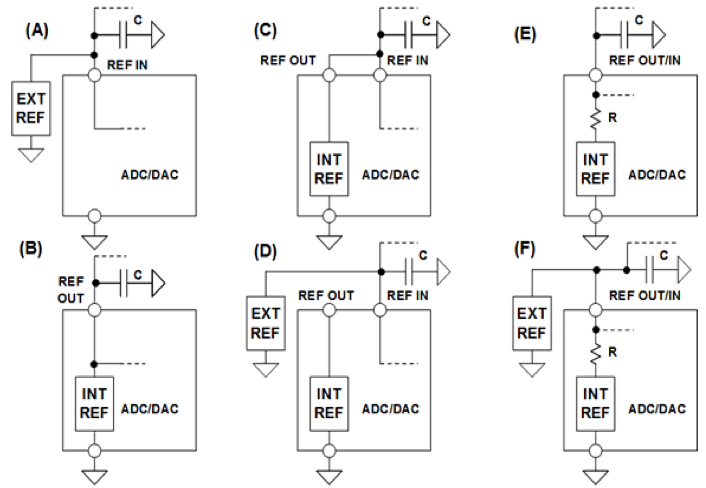
\includegraphics[scale=0.3]{images/variantenReferenzspannungen}
\end{figure}


\subsection{Verschiedene Arten der Rerferenzspannungserzeugung\hartl{276}} 
\begin{longtable}{|l|l|l|}
\hline
\begin{minipage}{4cm}
\textbf{Einfachste "`Referenzspannungsquelle"'}
\end{minipage}
&
\begin{minipage}{6cm}
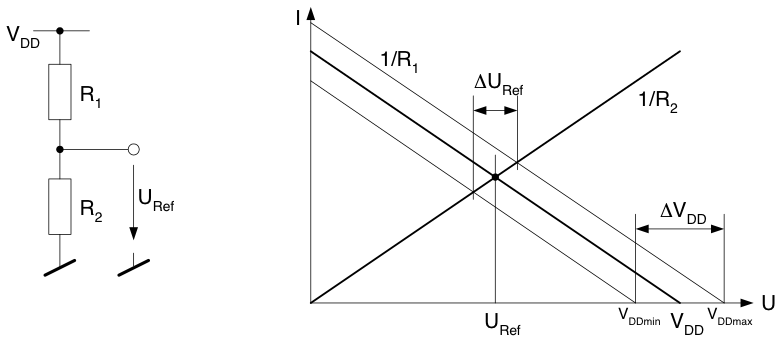
\includegraphics[width=6cm, height = 4cm]{images/spannungsteiler}
\end{minipage}
&
\begin{minipage}{8cm}
\begin{equation*}
S_{V_{DD}}^{U_{Ref}}=\frac{\frac{\Delta
U_{Ref}}{U_{Ref}}}{\frac{\Delta V_{DD}}{V_{DD}}}=1
\end{equation*}
\begin{itemize}
  \item S: Sensitivität
\end{itemize}
\end{minipage}
\\
\hline
\begin{minipage}{4cm}
\textbf{Dioden Referenz} \hartl{277}
\end{minipage}
&
\begin{minipage}{6cm}
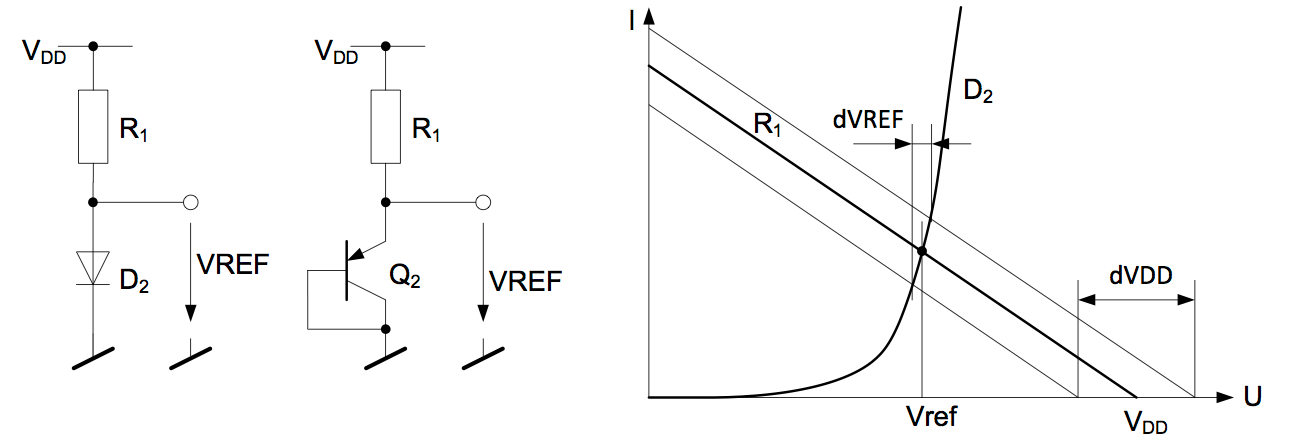
\includegraphics[width=6cm, height = 4cm]{images/diodenReferenz}
\end{minipage}
&
\begin{minipage}{8cm}
\begin{gather*}
U_{Ref}=U_{EB}=\frac{kT}{e}\ln{\frac{I}{I_{s}}} \notag\\\text{ für }V_{DD}>>
U_{EB}\\
S_{V_{DD}}^{U_{Ref}}=\frac{1}{\ln{\frac{I}{I_{S}}}}<1
\end{gather*}
\end{minipage}
\\
\hline
\begin{minipage}{4cm}
\textbf{MOSFET Referenz}
\end{minipage}
&
\begin{minipage}{6cm}
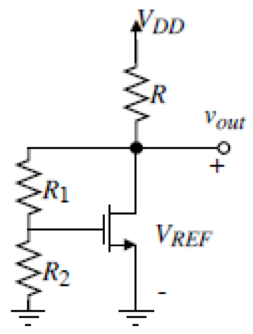
\includegraphics[width=4cm, height = 4cm]{images/mosfetReferenz}
\end{minipage}
&
\begin{minipage}{8cm}
\begin{equation*}
V_{REF}\approx \frac{R_{1}+R_{2}}{R_{2}}V_{GS}
\end{equation*}
\end{minipage}
\\
\hline
\begin{minipage}{4cm}
\textbf{Bootstrap Referenz}
\end{minipage}
&
\begin{minipage}{6cm}
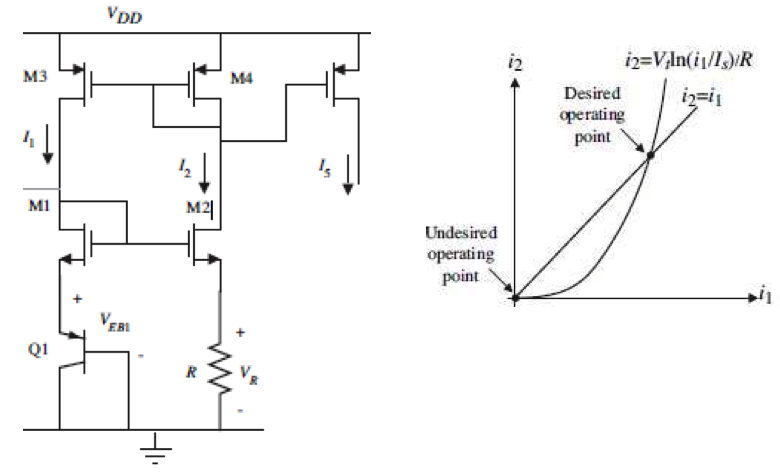
\includegraphics[width=6cm, height = 4cm]{images/bootstrapReferenz}
\end{minipage}
&
\begin{minipage}{8cm}
\begin{gather*}
I_{R}=I_{D}\\
I_{R}R=U_{T}\ln{\frac{I_{D}}{I_{S}}}\\
U_{T}=\frac{kT}{q}
\end{gather*}
\begin{itemize}
  \item Stromspiegel
  \item $U_{T}$: Temperaturabhängigkeit
\end{itemize}
\end{minipage}
\\
\hline
\begin{minipage}{4cm}
\textbf{Bandgap Referenz} \hartl{278}
\end{minipage}
&
\begin{minipage}{6cm}
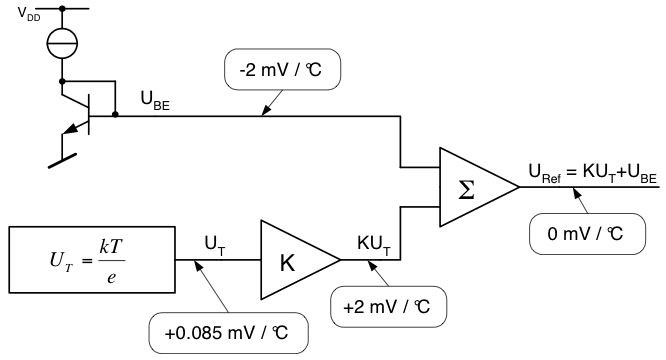
\includegraphics[width=6cm, height = 4cm]{images/bandgapReferenz1}\\
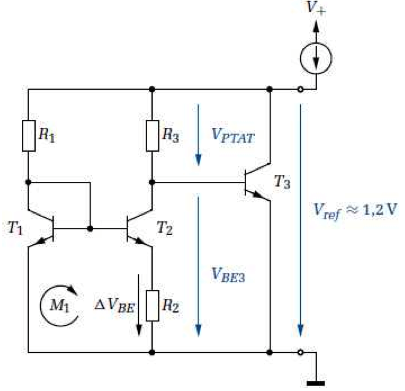
\includegraphics[width=6cm, height = 4cm]{images/bandgapReferenz2}
\end{minipage}
&
\begin{minipage}{8cm}
\begin{gather*}
	I_{C} = B*I_{BS}(e^{\frac{V_{BE}}{V_{T}}}-1)
		  \approx B*I_{BS}*e^{\frac{V_{BE}}{V_{T}}}\\
	\frac{I_{C1}}{I_{C2}} = e^{\frac{V_{BE1}-V_{BE2}}{V_{T}}} \\
	\Delta V_{BE}	= V_{BE1}-V_{BE2} = V_{T}\ln{\frac{I_{C1}}{I_{C1}}}\\
	V_{T} = \frac{kT}{q}\\
	 V_{BE3}+V_{PTAT}\approx{!}1,2V
\end{gather*}
\end{minipage}
\\
\hline
\begin{minipage}{4cm}
\textbf{Zenerdiode Referenz}
\end{minipage}
&
\begin{minipage}{6cm}
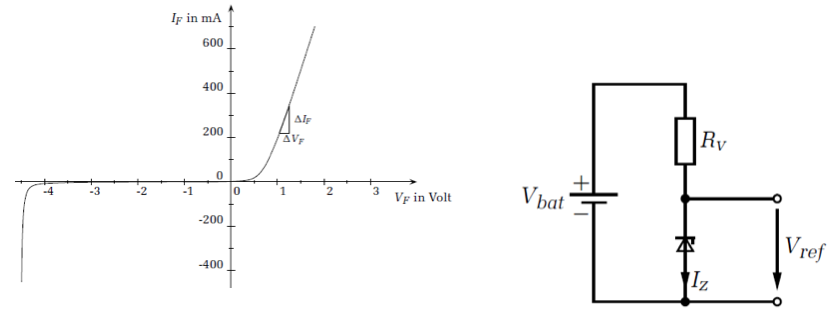
\includegraphics[width=6cm, height = 4cm]{images/zenerReferenz}
\end{minipage}
&
\\
\hline
\end{longtable}

